
\documentclass{beamer}
\usepackage{graphicx}
\usepackage{float}
\usepackage{hyperref}
\usepackage{ulem}
\usepackage{listings}
\usepackage{xcolor}

\definecolor{codegreen}{rgb}{0,0.6,0}
\definecolor{codegray}{rgb}{0.5,0.5,0.5}
\definecolor{codepurple}{rgb}{0.58,0,0.82}
\definecolor{backcolour}{rgb}{0.95,0.95,0.92}

\lstdefinestyle{mystyle}{
    backgroundcolor=\color{backcolour},
    commentstyle=\color{codegreen},
    keywordstyle=\color{magenta},
    numberstyle=\tiny\color{codegray},
    stringstyle=\color{codepurple},
    basicstyle=\ttfamily\tiny,
    breakatwhitespace=false,
    breaklines=true,
    captionpos=b,
    keepspaces=true,
    numbers=left,
    numbersep=5pt,
    showspaces=false,
    showstringspaces=false,
    showtabs=false,
    tabsize=2
}

\lstset{style=mystyle}

\hypersetup{
colorlinks=true,
linkcolor=blue,
filecolor=magenta,
urlcolor=cyan,
}

\urlstyle{same}

\title{Presentation}
\date{\today}
\author{Your Name Here}
\begin{document}
\frame{\titlepage}

\begin{frame}[fragile]
    \frametitle{Title of slide 1}

You can put regular text paragraphs here. Moreover, you can \textbf{bold your text} or \emph{italicize it} very
easily. Alternatively, you can use bullet points:


\begin{itemize}
\item Item 1
\item Item 2

\begin{itemize}
\item Item 2.2

\begin{itemize}
\item Item 2.2.1

\end{itemize}
\item Item 2.3

\end{itemize}

\end{itemize}


You can also write equations as you would in latex

$$
e^{i \pi} - 1 = 0
$$


\end{frame}


\begin{frame}[fragile]
    \frametitle{Title Slide 2}


    \begin{figure}
        \centering
        
\includegraphics[width=0.9\paperwidth,height=0.7\paperheight,keepaspectratio]{./figs/stock_image.jpg}
        \caption{You can fullscreen pictures with captions!}
    \end{figure}
\end{frame}


\begin{frame}[fragile]
    \frametitle{Pictures with text are automatically vertically split}

	\begin{minipage}{0.4\textwidth}
When you have a picture with text on the same slide, the area is automatically split.
\begin{itemize}
\item Margins can easily be adjusted in .tex file

\end{itemize}

	\end{minipage}%
	\hfill
	\begin{minipage}{0.55\textwidth}

    \begin{figure}
        \centering
        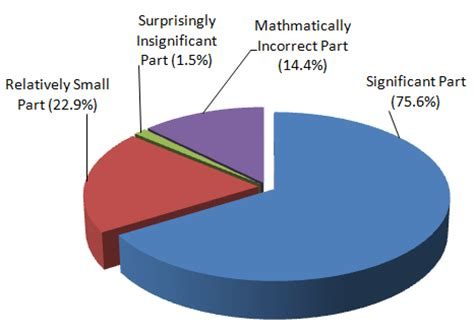
\includegraphics[width=\textwidth]{./figs/pie_chart.jpg}
        \caption{Anoter figure caption here!}
    \end{figure}	\end{minipage}

\end{frame}


\begin{frame}[fragile]
    \frametitle{Automatic Code Highlighting}

\begin{lstlisting}[language=python]
import matplotlib.pyplot as plt
def plot_data(x,y, title):
    plt.scatter(x,y)
    plt.title(title)
    plt.savefig("figure.png")

if __name__ == "__main__":
    print("plotting data")
    plot_data(list(range(5)), [20,15,6,9,10])
\end{lstlisting}


\end{frame}


\begin{frame}[fragile]
    \frametitle{In multiple languages!}

\begin{lstlisting}[language=fortran]
! calculate the kinetic energy of a flowfield
subroutine calculate_energy(energy)
    use m_work ! wrk arrays for velocity
    use m_parameters ! dx, dy, dz

    implicit none
    integer:: i, j, k
    real*8 :: energy, u, v, w

    energy = 0

    do i =1,nx
        do j=1,ny
            do k=1,nz
                u = wrk(i,j,k,1)
                v = wrk(i,j,k,2)
                w = wrk(i,j,k,3)

                energy = energy + u**2 + v**2 + w**2
            end do
        end do
    end do

    energy = energy * dx * dy * dz * 0.5

end subroutine calculate_energy
\end{lstlisting}


\end{frame}



\end{document}